\chapter{SourceMeter}\label{chap:SourceMeter}

\section{SourceMeter bevezetés}

\noindent

A SourceMeter egy forráskód-elemző eszköz, amely képes mély statikus programelemzést végezni a C, C++, Java, Python, C\#, JavaScript, TypeScript és RPG (AS/400)$^{~\cite{szHoke2014case}}$
nyelvű összetett programok forráskódján.
A FrontEndART a Szegedi Tudományegyetem Szoftverfejlesztés Tanszékén kutatott és fejlesztett Columbus technológián$^{~\cite{beszedes2005columbus}}$ alapuló SourceMeter eszközt fejlesztette ki.
A statikus kódelemzés egy olyan módszer, amely során a program forráskódját elemezzük, anélkül hogy azt ténylegesen futtatnánk.
Az elemzés során különböző eszközök segítségével ellenőrizhetjük a kód helyességét, hatékonyságát, biztonságosságát és karbantarthatóságát.
Az ilyen típusú elemzés során gyakran felhasználnak különböző szabályokat és előírásokat, amelyek segítenek az azonosításban és a hibák javításában.

\noindent

A statikus elemzés során absztrakt szemantikus gráf (ASG) készül a forráskód nyelvi elemeiből.
Ezután az ASG-t különböző eszközökkel dolgozzák fel a csomagban annak érdekében, hogy kiszámítsák a metrikákat (LLOC$^{~\cite{siket2014differences}}$, NLE vagy NOA),
azonosítsák az ismételt kódrészleteket (másolás-beszúrás; klónok), a kódolási szabályszegéseket, stb.
A SourceMeter képes elemzést végezni olyan forráskódon,amely megfelel a Java 8 és korábbi verzióinak, a C/C++,
az RPG III és az RPG IV verzióinak (beleértve a szabadon formázottakat), a C\# 6.0 és korábbi verzióinak, valamint a Python 2.7.8 és korábbi verzióinak.
A C/C++ esetében a SourceMeter támogatja az ISO/IEC 14882:2011$^{~\cite{sourcemeter2015}}$ nemzetközi szabványt, amelyet kiegészítettek az ISO/IEC 14882:2014 új funkcióival, és a C nyelvet az ANSI/ISO 9899:1990, az ISO/IEC 9899:1999 és az ISO/IEC 9899:2011 szabványok határozzák meg.
Az alapértelmezett funkciókon túl, a GCC és a Microsoft által meghatározott kiterjesztések is támogatottak.

\noindent

A SourceMeter a QualityGate$^{~\cite{bakota2014qualitygate}}$ eszközben van használva.

\noindent

A SourceMeternek található egy plug-in a SonarQubehoz.
A SourceMeter plug-in a SonarQube platformhoz egy kiterjesztése az nyílt forráskódú SonarQube platformnak, amelyet a kód minőségének kezelésére használnak
A plug-in a SourceMeter-t futtatja a SonarQube platformról, és feltölti a forráskód elemzésének eredményeit a SourceMeter-től a SonarQube adatbázisába.
A plug-in nyílt forráskódú, és az összes szokásos SonarQube kódelemzési eredményt biztosítja, kiegészítve sok további metrikával és problémakeresővel, amelyeket a SourceMeter eszköz biztosít.
A plug-in támogatja a C/C++, a Java, a C\#, a Python és a RPG nyelveket.$^{~\cite{ferenc2014source}}$

\section{SourceMeter for JavaScript}

\noindent

A SourceMeter for JavaScript a SourceMeternek egy nagyobb alprojektje.
A SourceMeter for JavaScript egy olyan eszköz, amely lehetővé teszi a mély statikus forráskód elemzést a bonyolult JavaScript és TypeScript rendszerekben.
Képes felismerni a kód hibáit, mint például a nem definiált változók vagy függvények használata, a nem biztonságos kódrészletek, a nem hatékony kódrészletek, valamint a redundáns és ismétlődő kódok.
Ezenkívül az eszköz képes összehasonlítani a kódot az általános gyakorlatokkal és a meghatározott szabályokkal, és jelezni az eltéréseket.
Az ilyen eszközök használata segíthet az észlelt hibák javításában és a kód minőségének javításában, ami végső soron javíthatja a rendszer biztonságát és hatékonyságát.

\noindent

A SourceMeter for JavaScript projekt több alprojektet is magába foglal, amelyek különböző részfeladatokra specializálódnak.

\subsection{Nyelvi séma bevezetés}\label{chap:nyelvi_sema}
A JavaScript nyelvi séma(továbbiakban: séma)$^{~\cite{ferenc2002columbus}}$  egy UML Diagramhoz hasonlító séma.
A Visual Paradigm(továbbiakban: vpp) alkalmazással szerkeszthető.
Azért szerkesztjük a sémát vpp-ben, mivel a többi nyelvi változat esetében is így volt, és van koncerter, ami ebből a vpp fájlból létrehozza a C++ alap fájlokat, amiket az elemző programok tudnak használni.
A felépítése a következőképpen néz ki:

\begin{figure}[!htbp]
      \caption{Séma struktúrális felépítése}\label{fig:JavaScriptSchema_struktura}
      \centering
      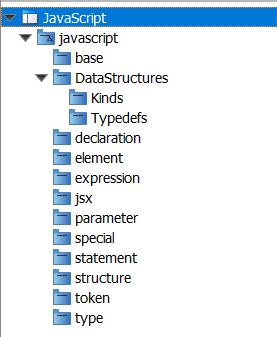
\includegraphics[width=0.4\textwidth]{JavaScriptSchema_struktura.png}
\end{figure}

\Aref{fig:JavaScriptSchema_struktura} ábrán a ProjektNlv/Model/Package-ek struktúra figyelhető meg.
A projekt neve JavaScript, ezen belül található egy model, amit javascript-nek hívnak.
A modellen belül találhatóak meg a package-ek.
A Package-ek a TypeScript séma $^{~\cite{typescript-eslint}}$ alapján lettek elnevezve.
Átláthatóság és könnyebb bővíthetőség szempontjából lett létrehozva több package.
Követtük a TypeScript-eslint$^{~\cite{typescript-eslint}}$ projekt struktúrális felépítését.
A package-ek a következőképpen épülnek fel:
\begin{figure}[!htbp]
      \caption{A base package felépítése}\label{fig:base_vpp}
      \centering
      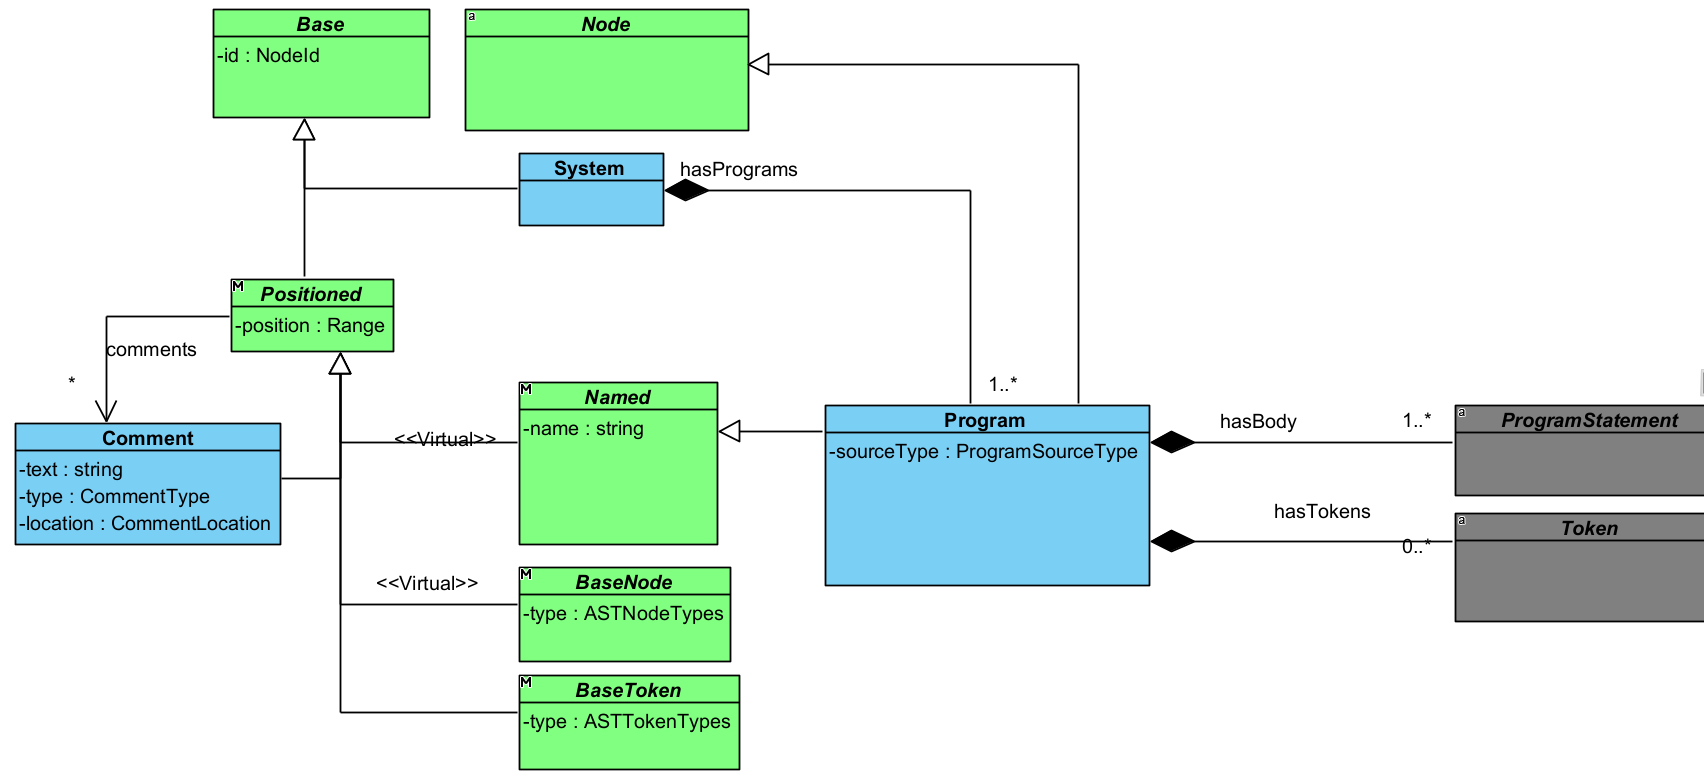
\includegraphics[width=0.9\textwidth]{base_vpp.png}
\end{figure}

\Aref{fig:base_vpp} ábrán a Base, Node, Positioned, Comment, System, Named, BaseNode, BaseToken, Program, ProgramStatement és a Token osztályok találhatóak.
A Base osztályból öröklődik minden osztály.
A Base osztály rendelkezik id attribútummal, ami NodeId típusú.
Az absztrakciót zöld háttérszínnel jelöltük.
A séma könnyebb bővíthetősége és olvashatósága miatt jeleztük így, illetve más nyelvi sémákban is ezt a logikát követjük.
Más package-ekben lévő definiálást szürke háttérszínnel, ugyanabban a package-ben lévő definiálást világosszürke háttérszínnel jelöltük.
Az alapértelmezett osztályt kék háttérszínnel jelöltük.
A Positioned osztályból öröklődnek a Named, BaseNode és a BaseToken osztályok.
A BaseNode osztályból több minden öröklődik, mint például a DeclarationStatement, ImportDeclaration, Expression és több minden is. Ez látható \aref{fig:declaration_vpp} ábrán.
A Positioned osztály rendelkezik position attribútummal, ami Range típusú. A Positioned osztályhoz tartozhatnak kommentek is.
A Comment osztály öröklődik a Positioned osztályból, ezzel biztosítva azt, hogy minden kommentnek lesz pozíciója.
A Comment osztály rendelkezik text, type és location attribútummal.
A CommentType és a CommentLocation a DataStructures package-ben lett definiálva.
Végül, Program osztály öröklődik a Named osztályból, ezáltal rendelkezik name attribútummal, ami string típusú.
Minden Program osztályhoz tartozik legalább 1 System, ezt az 1..*-al jelöltük.
A hasPrograms-nak a JavaScriptAddon-ban van jelentősége.
A ProgramSourceType is a DataStructures package-ben lett definiálva. A ProgramSourceType értéke lehet source, vagy module.
A Base package eltér a TypeScript-eslint$^{~\cite{typescript-eslint}}$ projektben lévő Base package-től.
Régebbi sémának a Base package-ét használjuk, BaseNode és BaseToken osztályok kibővítésével.

\noindent

Mivel a Base package egyedi a mi esetünkben, ezért kitérnék a Declaration package-re is.
A Declaration package-n belül az ExportAllDeclaration osztályt mutatom be.

\begin{lstlisting}[caption={ExportAllDeclaration TypeScript megvalósítása},label={lst:ExportAllDeclaration}, language={JavaScript}]
export interface ExportAllDeclaration extends BaseNode {
      type: AST_NODE_TYPES.ExportAllDeclaration;
      assertions: ImportAttribute[];
      exported: Identifier | null;
      exportKind: ExportKind;
      source: StringLiteral;
}
\end{lstlisting}

\Aref{lst:ExportAllDeclaration} kódrészlet megvalósítása a sémában:

\begin{figure}[!htbp]
      \caption{A Declaration package felépítése}\label{fig:declaration_vpp}
      \centering
      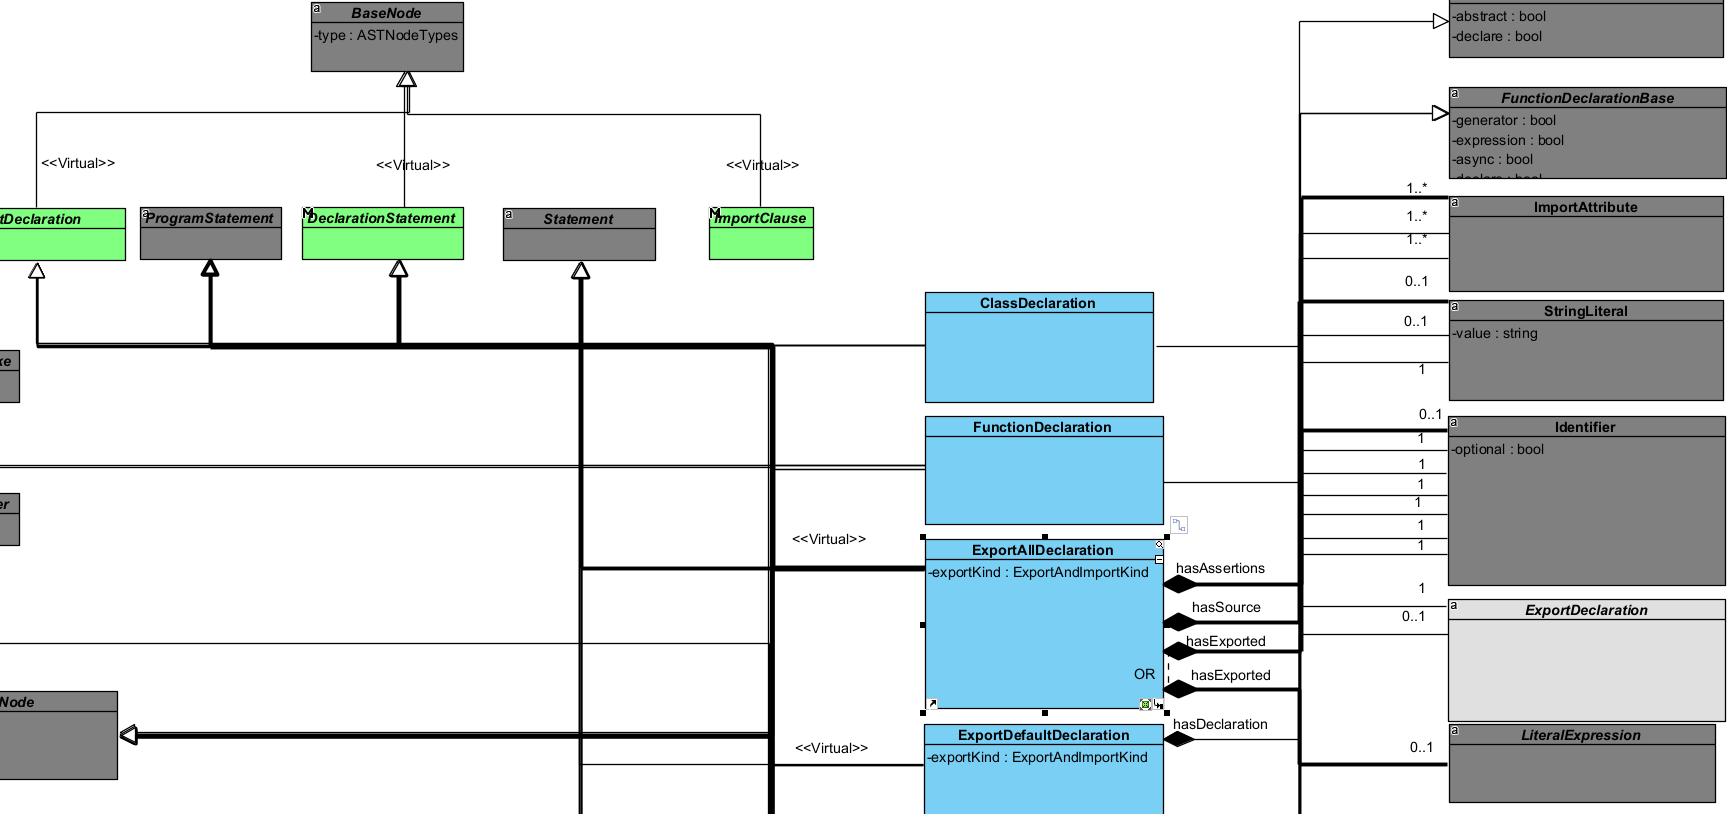
\includegraphics[width=1\textwidth]{declaration.png}
\end{figure}

Az ExportAllDeclaration osztály öröklődik a DeclarationStatement osztályból, ami öröklődik a BaseNode osztályból.
Ezért az ExportAllDeclaration egyaránt öröklődik a BaseNode osztályból.
\Aref{lst:ExportAllDeclaration} kódrészletben ez az extends BaseNode-al van jelezve.
A főbb osztályok a BaseNode alatt találhatóak az ábrán.
Az ábra jobb oldalán lévő osztályok, amik sötét- és világosszürkével vannak jelölve, az attribútumok.
Az ExportAllDeclaration osztály öröklődik a Statement, DeclarationStatement, Node és a ProgramStatement osztályokból.
Az összes öröklődés a TypeScript-eslint$^{~\cite{typescript-eslint}}$ projekt unions mappájában találhatóak meg.
Az ExportAllDeclaration osztály rendelkezik pozíció, Comment, type és NodeId attribútummal, mivel öröklődik a BaseNode osztályból.
Emellett még rendelkezik Assertions, Source és Exported attribútummal is.
Az Assertions attribútum típusa ImportAttribute, amihez legalább egy ImportAttribute tartozik.
Az Exported attribútumnál típusa lehet vagy Identifier vagy LiteralExpression.
A vagyolást egy OR-ral jeleztük a sémában.
Az Exported attribútum opcionális, ezért az értéke lehet null is. Ezt a sémában a 0..1-el jelöltük.
A Source attribútum is opcionális, típusa StringLiteral.
Végül, ExportKind attribútummal is rendelkezik, típusa ExportAndImportKind.
Az ExportAndImportKind az a DataStructures package-ben lett definiálva.
Így lett minden package és osztály felépítve.
A DeclarationStatement, Statement, ProgramStatement és több osztály, ami a unions mappában található, gyűjtő osztály, aminek a jelentősége a JavaScriptAddon-nál fog mutatkozni.

\noindent

A DataStructures package többször volt említve, hadd mutassam be a következő ábrán a felépítésést:

\begin{figure}[!htbp]
      \caption{A DataStructures package felépítése}\label{fig:data_structures_kinds}
      \centering
      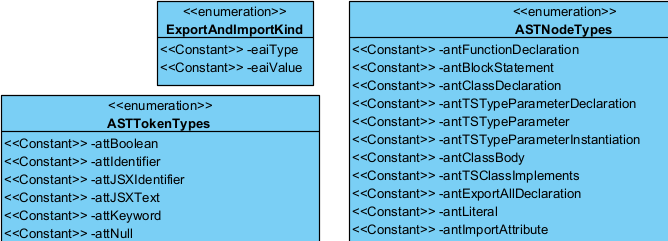
\includegraphics[width=0.8\textwidth]{data_structures.png}
\end{figure}

A DataStructures package-ben található 2 package, Kinds és Typedefs. \Aref{fig:JavaScriptSchema_struktura} ábrán látható. Ebből a Kinds package-et mutatom be.
\Aref{fig:data_structures_kinds} ábrán a Kinds package-nek egy kisebb része látható.
Enumok vannak deklarálva ebben a package-ben.
Az enumokban konstansok találhatóak. Minden konstans előtt található 3 karakter, ezek a karakterek ASG konvertáláskor el fognak tűnni.
Ha ExportAndImportKind-ot adunk meg egy attribútum típusának, akkor az attribútum típusa lehet Type vagy Value.

\noindent

Ahhoz, hogy tudjuk használni a sémát, először ki kell exportálni. Ezt a vpp segítségével tehetjük meg, egy xml formátumú fájlba exportáljuk az egész projektet.
Ezután ezt a fájlt átkonvertáljuk egy asg kiterjesztésű fájlra.
A SourceMeter alprojektei közé tartozik egy úgynevezett UmlToAsg.
Ez a projekt egy xml fájlból egy asg fájlt generál.
Az UmlToAsg projektet a SchemaGenerator segítségével tudjuk legenerálni.
A SchemaGenerator C++ nyelven megírt eszköz.
Több mindent is generál C, C++, vagy Java nyelven.
A SchemaGenerator is a SourceMeter alprojektei közé tartozik.
A legenerált asg fájl elején a következő sorok láthatóak:

\begin{lstlisting}[caption={Asg fájl első sorai},label={lst:asg_file_eleje}, language={JavaScript}]
NAME = javascript;
APIVERSION = 0.3.1;
BINARYVERSION = 0.3.1;
CSIHEADERTEXT = JavaScriptLanguage;
\end{lstlisting}

A verziókat kézzel tudjuk átírni abban a fáljban ami generálja ezt, ez egy C++ fájl, a SchemaGeneratorban található meg.
Ezután a Kinds package tartalmát írja bele a következőképpen:

\begin{lstlisting}[caption={Asg fájl kind},label={lst:asg_file_kinds}, language={JavaScript}]
KIND ASTNodeTypes (ant) {
      FunctionDeclaration;
      BlockStatement;
      ClassDeclaration;}
\end{lstlisting}

A 3 karaktert, amit minden konstans elé írtunk, kikerült paraméterbe és csak az utáni stringet írta át.
Ugyanígy jár el a többi enumnál is.
Ha az összes enumot beleírta, akkor a többi package-et kezdi el bele írni a fájlba. \Aref{fig:JavaScriptSchema_struktura} alapján megy sorba.
Példának a Declaration package-et mutatom be, azon belül is az ExportAllDeclaration osztályt.

\begin{lstlisting}[caption={Asg fájl ExportAllDeclaration},label={lst:asg_file_export_all_declaration}, language={JavaScript}]
SCOPE declaration {
      NODE DeclarationStatement : virtual base::BaseNode [ABSTRACT] {
      }
      NODE ExportAllDeclaration : DeclarationStatement, statement::Statement, virtual statement::ProgramStatement, special::Node {
            ATTR ExportAndImportKind exportKind;
            EDGE TREE 1 hasExported (expression::Identifier | expression::LiteralExpression);
            EDGE TREE 1 hasSource (structure::StringLiteral);
            EDGE TREE * hasAssertions (special::ImportAttribute);
      }
}
\end{lstlisting}

Az UmlToAsg minden egyes package-et Scope-nak értelmez.
A Scope-on belül az osztályokat gráf csomópontnak (továbbiakban: node) értelmezi.
A node-nak kettő különféle attribútuma lehet, ATTR és EDGE TREE.
Akkor konvertálja ATTR-ra az attribútumot, ha az a DataStructures package-ben deklarálva lett. Egyéb esetben EDGE TREE-vé konvertál.
Az EDGE TREE után álló szám vagy csillag, az adott attribútum multiplicitását jelenti.
A vagyolást egy | jellel jelzi.
Az öröklődést kettősponttal jelzi.
Felsorolásszerűen írta át, ha valami másból származik, akkor packageNev::osztalyNev szerint.
\Aref{fig:declaration_vpp}as ábrán látható, hogy mit hogyan írt át.

\subsection{JavaScriptAddon bevezetés}\label{chap:javaScriptAddon_bevezetes}

\noindent

A JavaScriptAddon a SchemaGenerator által generált fájl.
\Aref{lst:asg_file_export_all_declaration} kódrészleten látható, hogy node-okat generált az UmlToAsg az osztályokból.
Ezeknek a node-oknak a SchemaGenerator generál külön egy WrapperHeader és egy WrapperCC fájlt.
A SchemaGenerator továbbá generál Factory.cc és a hozzátartozó header fájlt. A Factory.cc-t bővebben taglalom \aref{lst:factory_cc} kódrészletnél.
A WrapperCC, Factory.cc és a hozzájuk tartozó header fájlok összeolvasztása eredményezi a JavaScriptAddon fájlt.
A JavaScriptAddon fájl generálás menetét a NodeAddonGenerator fájlban írjuk le.
A SchemaGenerator main.c fájlba beimportáljuk a NodeAddonGenerator összes metódusát, aztán ezeket a metódusokat használva legeneráljuk a JavaScriptAddon fájlt.
A $-genNodeAddon$ kapcsolóval fogja legenerálni a JavaScriptAddon fájl a SchemaGenerator.
A SchemaGenerator main.c fájl elején előszőr vizsgál a megadott kapcsolókra az alábbi módon:

\begin{lstlisting}[caption={SchemaGenerator kapcsoló vizsgálás},label={lst:schemagenerator_argv_genNodeAddon}, language={CStyle}]
if(!strcmp(argv[i], "-genNodeAddon")){
      options.generateNodeAddon = true;
}
\end{lstlisting}

Ha az argumentumban megtalálható a genNodeAddon, akkor az options.generateNodeAddon-t igazra állítja.
Az alapértelmezett értéke az options.generateNodeAddon-nak hamis.
Több fájl generálás után, ami kell több program működéséhez, megvizsgálja az options.generateNodeAddon-t.
Ha az options.generateNodeAddon hamis, akkor nem fog semmi se történni.

\begin{lstlisting}[caption={SchemaGenerator JavaScriptAddon generálás},label={lst:schemagenerator_genNodeAddon_check}, language={CStyle}]
if (createAndEnterDirectory(SOURCE_NODE_ADDON_DIR_NAME)) {
      generatePackageJson();
      generateBindingGyp();
      generateAddonCC();
      generateFactoryWrapper();
      if (createAndEnterDirectory("inc")) {
            generateWrapperHeaders();
            leaveDirectory();}
      if(createAndEnterDirectory("src")){
            generateWrapperSources();
            leaveDirectory();}
leaveDirectory();}
\end{lstlisting}

A createAndEnterDirectory metódus először létrehoz egy addon nevű mappát és chdir parancsot használva belelép.
Ha ez a mappa már létezik, akkor a létrehozást kihagyja és a chdir paranccsal belelép.
Létrehozás és chdir parancs használat után az addon mappába generál package.json fájlt.
Ebben a fájlban beállítja a projekt nevét, verziószámát, függőségeket, szkripteket és a gypfájl kapcsolónak igaz értéket beállítja.

\begin{lstlisting}[caption={NodeAddonGenerator package.json szkriptek}, label={lst:nodeAddonGenerator_package_json}, language={CStyle}]
fprintf(f, "    \"rebuild\": \"node-gyp configure && node-gyp rebuild -j 8\",\n");
fprintf(f, "    \"install\": \"node-gyp configure && node-gyp build -j 8\"\n");
\end{lstlisting}

\Aref{lst:nodeAddonGenerator_package_json} kódrészleten látható, hogy a node-gyp build segítségével fog történni a buildelés.
A node-gyp egy eszköz, amely összeállítja a Node.js Addonokat. A Node.js Addonok natív Node.js modulok, amelyeket C vagy C++ nyelven írnak.
Miután az ilyen modulokat eszközökkel, például a node-gyppel lefordították, funkcióik elérhetők lesznek a $require()$ segítségével, ahogy bármely más Node.js modul esetében.

\noindent

A package.json fájl után generálja le a binding.gyp fájlt.
A binding.gyp fájlban találhatóak meg az összes node fájl relatív útvonala a package.json fájlhoz képest.
A binding.gyp fájl után generálja le az addonCC fájlt.

\begin{lstlisting}[caption={Addon.cc Wrapperek importolása}, label={lst:addoncc_wrapper_include}, language{CStyle}]
if (!traversalDescendantBFT(rootNode, generateWrapIncludes, false)) {
      debugMessage(0, " failed\n");
      fclose(f);
      return false;
}
\end{lstlisting}

A traversalDescendantBFT metódus egy bejárás, ami az összes node-ra lefut. Ezekre a node-okra meghívja a generateWrapIncludes metódust.
A generateWrapIncludes metódus a NodeAddonGenerator fájlban van leimplementálva a következőképp:

\begin{lstlisting}[caption={generateWrapIncludes leimplementálása}, label={lst:addoncc_wrapper_includes_implementation}, language{CStyle}]
if(node->type.abstract){
      return true;
}
fprintf(f, "#include \"");
fprintf(f, "inc/%sWrapper.h\"\n", node->name );
return true;
\end{lstlisting}

Ha a jelenlegi node absztrakt, akkor nem ír semmit a fáljba.
Ha nem absztrakt, akkor \aref{lst:addoncc_wrapper_includes_implementation} kódrészlet alapján importálja a node-nak a header fájl relatív útvonalát.
A \texttt{node->name} több értéket is vehet fel, például FunctionDeclaration, ClassDeclaration, ezek megtalálhatóak az asg fájlban.
Ezután ez a bejárás még egy alkalommal végrehajtódik. Ebben az esetben a wrapperIniteket ír az addonCC fájlba.

\begin{lstlisting}[caption={generateWrapInit leimplementálása}, label={lst:addoncc_wrapper_inits_implementation}, language={CStyle}]
fprintf(f, "  columbus::%s::asg::addon::%sWrapper::Init(env, exports);\n", schemaName, node->name);
\end{lstlisting}

\noindent

Az addonCC fájl generálása után a generateFactoryWrapper függvényhívás történik.
Ebben a függvényben 2 metódus függvényhívás található, a generateFactoryWrapperHeader és generateFactoryWrapperSource.

\noindent

A generateFactoryWrapperHeader a Factory.h fájlt generálja le.
Először importálja az összes nodeWrapper header fájlt, és utána létrehoz egy Factory osztályt, a publikus metódusait, ami az Init és Destructor, illetve a private metódusait,
ami a destructor, New, SaveAST, LoadAST, Clear, getRoot és az összes nodeWrapper create metódusai.

\noindent

A generateFactoryWrapperSource a Factory.cc fájlt generálja le.
DECLARE\_NAPI\_METHOD-okat hoz létre, az összes nodeWrapper fájlnak.

\begin{lstlisting}[caption={Factory.cc fájl}, label={lst:factory_cc}, language={CStyle}]
napi_property_descriptor props [] = {
      DECLARE_NAPI_METHOD("getRoot", getRoot),
      DECLARE_NAPI_METHOD("createCommentWrapper", createCommentWrapper)
      ...}
\end{lstlisting}

\noindent

Legvégül, a SchemaGenerator legenerálja az inc és az src mappákat.
Az inc mappában találhatóak a header fájlok minden egyes nodeWrapper-nek, az src mappában maguk a nodeWrapper-ek vannak megvalósítva.

\noindent

A SchemaGenerator legenerálj az ExportAllDeclarationWrapper.h és az ExportAllDeclaration.cc fájlokat.
A header fájlban létrehozza az ExportAllDeclarationWrapper osztályt, ami öröklődik a BaseWrapperből. A BaseWrapper alap Wrapper osztály.
Három publikos metódust generál le, az Init-et, a Destructor-t és a NewInstance-t.
Ezen felül több private metódust is.

\begin{lstlisting}[caption={ExportAllDeclarationWrapper.h fájl}, label={lst:ExportAllDeclarationWrapper_header}, language={CStyle}]
napi_property_descriptor props [] = {
      static napi_value setPosition(...);
      static napi_value addAssertions(...);
      static napi_value setType(...);
...}
\end{lstlisting}

\Aref{lst:ExportAllDeclarationWrapper_header} kódrészleten megfigyelhető, hogy létrehozott az ExportAllDeclarationWrapper-nek egy setPosition, addAssertions, setType metódusokat.
Ezek az ExportAllDeclaration attribútumai, ami a sémában be lett állítva.
\Aref{fig:declaration_vpp} ábrán látható, hogy az ExportAllDeclaration hasAssertions attribútumának a multiplicitása 1..*, ezt átkonvertálta addAssertions-re.
Ahol 0..* a multiplicitás, azt átkonvertálta setAttribute-ra, például setSource vagy setExported-re.
Minden nodeWrapper rendelezik setPath, setPosition, setType és addComments metódusokkal.

\noindent

Az ExportAllDeclaration.cc fájlt ugyanúgy generálja le, mint a Factory.cc fájlt. DECLARE\_NAPI\_METHOD-okat generál, a setExported, setSource, setType és a többi metódushoz.
Ezután az összes metódust megvalósításra kerül.

\subsection{JSAN2Lim bevezetés}

\noindent

A JSAN2Lim C++ programozási nyelvben megírt program. A JSAN általi eredményt alakítja át nyelvfüggetlen (továbbiakban: LIM) formátumú fájlokra.
Azért LIM formátumú fájlokra alakít át, mivel egy nyelvfüggetlen modellen sokkal könnyebb metrikákat mérni.
A JSAN2Lim függ a JSAN programtól, hiszen a JSAN eredményeit alakítja át, tehát, ha a JSAN programot változás éri, akkor a JSAN2Lim programot is változtatni kell, különben nem lesznek pontosak a metrika mérések.
A JSAN2Lim használja a LimSchema-t. A LimSchema hasonlóan van felépítve, mint a JavaScript nyelvi sémája.
A JSAN2Lim bejárja az összes node-ot ami megtalálható a JSAN általi eredmény fájlban.
Minden node-ra külön meg kell írni a bejáró (továbbiakban: visit) függvényt.

\noindent

A JSAN2Lim működését egy kódrészleten keresztül mutatom be.
\begin{lstlisting}[caption={ClassDeclaration Visitor}, label={lst:classdeclaration_visitor}, language={CStyle}]
VISIT_BEGIN(clNode, callVirtualBase);
lim::asg::logical::Class& classLimNode = dynamic_cast<lim::asg::logical::Class&>(createLimNode(clNode, callVirtualBase));
fillData(classLimNode, clNode);//sets the name
fillMemberData(classLimNode);
demangledNameParts.push_back(classLimNode.getName());
classStack.push(ClassInfo());
classStack.top().classNodeId = classLimNode.getId();
if (clNode.getSuperClass() != NULL) {
      if (javascript::asg::Common::getIsIdentifier(*clNode.getSuperClass())) {
            javascript::asg::expression::Identifier& superClass = dynamic_cast<javascript::asg::expression::Identifier&>(*clNode.getSuperClass());
            classStack.top().isSubclass = superClass.getId();}}
if (!packageStack.empty()) {
      lim::asg::logical::Package& packageLimNode = dynamic_cast<lim::asg::logical::Package&>(limFactory.getRef(packageStack.top().packageNodeId));
      SAFE_EDGE(packageLimNode, Member, lim::asg::logical::Member, classLimNode.getId());}
addIsContainedInEdge(classLimNode, clNode);
\end{lstlisting}

A VISIT\_BEGIN a ViscitorAbstractNodes programnak a visit metódusa.
Ezután létrejön a classLimNode változó, ami \texttt{lim::asg::logical::Class\&} típusú.
Ez a típus a LimSchema-ban található meg, a logical package-ben.
A változónak a createLimNode metódus által visszaadott node lesz az értéke.
Ezt az értéket konvertáljuk át a erre a \texttt{lim::asg::logical::Class\&} típusra.

\noindent

A createLimNode függvény meghívja a createNode függvényt. Ez a függvény vár paraméterbe egy nodeKind-ot.
A nodeKind az adott node típúsát jelöli.
A nodeKind-ot a getLimKind függvény határozza meg.
A getLimKind függvény megvizsgálja, hogy az adott node \texttt{getIsClassDeclarationBase} vagy \texttt{getIsMethodDefinition} vagy \texttt{getIsFunctionDeclarationBase}.
A nodeKind értéke típustól függően adódik meg.
Ezek az értékek a következők lehetnek: ndkClass, ndkMethod, ndkParameter, ndkMethodCall, ndkAttribute, ndkComment, ndkPackage, ndkAttributeAccess, ndkComponent.
Ezek az értékek mind a LimSchema-ban vannak deklarálva. A nodeKind értékadása után a függvény visszaadja ezt a változót és tovább használja a visitor-ban.
Ezután, a createLimNode függvény létrehozza a megfelelő node-ot a nodeKind-tól függően. Beállítja a pozícióját a node-nak és visszaadja a *limNode-ot.

\noindent

Ebben az esetben a nodeKind az ndkClass értéket kapja meg.
A classLimNode értékadás után meghívódik a filldata függvény.
Kettő paramétert vár, classLimNode-ot, és a node-ot.
A filldata a JSAN általi adott eredményet bejárja, visitorok segítségével.
A filldata-ban beállítódik a limnode láthatósága, nyelve, az hogy absztrakt-e és a classKind-ja, ami jelen esetben clkClass értéket fog felvenni.

Ezután beállítódik a limnode neve. Ha a node-nak volt identifier-e, akkor a \texttt{getName} függvénnyel beállítódik a limnode neve különben \texttt{anonymousClass} érték állítódik be.
Ezután megvizsgálja, hogy a methodstack (ami egy stack és metódusokat tartalma) üres-e.
Ha nem üres, akkor létezik szülője, ezért a SAFE\_EDGE metódussal hozzáadódik egy csúcs a szülő és a jelenlegi limnode között.
Ezt uganúgy megvizsgálja a  packageStack-re (ami egy stack és csomagokat tartalmaz), ha nem üres, akkor ugyanezt elvégzem csak a szülő más lesz.
Legvégül az \texttt{addIsContainedInEdge} függvény meghívódik a limnode és a jsNode paraméterekkel.

\noindent

Ezután a \texttt{fillMemberData} függvény hívódik meg.
Ez a függvény a limnode pozícióját állítja be, és a nevén változtat.
Utána a classStack-hez hozzáadódik az adott osztály tulajdonságai, beállítja a szülő osztályt ha van, a pozícióját is beállítja, és a végén meghívódik az \texttt{addIsContainedInEdge} a classLimNode és a clNode paraméterekkel.
Minden egyes node-nál ez az eljárás fut le.

\subsection{Regressziós tesztelés bevezetés}

\noindent


A regressziós tesztelés általában egy olyan szoftvertesztelési típus, amely akkor használatos, amikor megerősítjük, hogy a legfrissebb program- vagy kódmódosítások nem érintették negatív módon a meglévő funkciókat.
A regressziós tesztelés során megállapítják, hogy a szoftver vagy alkalmazás megfelelően működik-e az új változások és hibajavítások tekintetében.
A regressziós tesztelés főként arról szól, hogy az már végrehajtott teszteseteket újra lefuttatjuk annak érdekében, hogy megerősítsük, az alkalmazás megfelelően működik-e.

A regressziós tesztelésnek 7 különböző típusa van:

\noindent

Re-test All (Mindent újratesztelni): Egy módja a regressziós tesztelésnek az, hogy az összes tesztesetet újra futtatjuk.
Ez valójában egy költséges folyamat, mivel több időt, erőforrást és erőfeszítést igényel az egész teszteset újbóli végrehajtása.
Az ebben a folyamatban észlelt hibákat előre jelentik a javítás érdekében.

\noindent

Corrective Regression Testing (Javító regressziós tesztelés):
A javító regressziós tesztelés a regressziós tesztelés egyszerűbb formái közé tartozik, minimális erőfeszítést igényel.
A javító regressziós tesztelés nem igényel változásokat a meglévő kódbázisban és az alkalmazásba új funkciók hozzáadását.
Egyszerűen csak a már meglévő funkciókat és azok teszteseteit kell tesztelni, és nem kell újakat létrehozni.

\noindent

Unit Regression Testing (Egység regressziós tesztelés):
Az egység regressziós tesztelés a regressziós tesztelés elengedhetetlen része, amelyben a kódot elszigetelve teszteljük.
Az integrációkat és függőségeket kikapcsoljuk az egység regressziós tesztelés során, és az egyes egységekre helyezzük a hangsúlyt.
Általában alacsony forgalmú és csúcsidőn kívül végzik ezt a tesztelést.

\noindent

Selective Regression Testing (Szelektív regressziós tesztelés):
A szelektív regressziós tesztelés elemzi a meglévő kódot és mind az új, mind a meglévő kód hatását.
A közös elemeket, mint a változókat és funkciókat, az alkalmazásba beillesztik, hogy gyors eredményeket kapjanak, anélkül, hogy befolyásolnák a folyamatot.

\noindent

Progressive Regression Testing (Progresszív regressziós tesztelés):
A progresszív regressziós tesztesetek az elvárások alapján készülnek.
Amikor csak kisebb termékfejlesztések vannak, az új teszteseteket úgy tervezik, hogy ne befolyásolják a termék meglévő kódját.

\noindent

Complete Regression Testing  (Teljes regressziós tesztelés):
Néhány kisebb vagy jelentős változtatásnak hatalmas hatása lehet a termékre.
A teljes regressziós tesztelést ebben az esetben használják, amikor jelentős módosítások vannak a jelenlegi kódban.
Segít a tesztelési folyamat során történt bármilyen módosítás javításában.

\noindent

Partial Regression Testing (Részleges regressziós tesztelés):
Amikor új kód kerül hozzáadásra egy meglévő kód bázishoz, akkor a részleges regressziós tesztelést alkalmazzák.
Ez segít felfedezni a kritikus hibákat a meglévő kódban, és lehetővé teszi a tesztelést anélkül, hogy a rendszer működését befolyásolná.
